\documentclass[11pt]{article}
\usepackage[margin=1in]{geometry}
\usepackage[pdftex]{graphicx}
\usepackage{amsmath,amssymb,amsthm}
% Same reason as the F = ma FAQ: microtype's font expansion needs scalable
% faces, so load Latin Modern before anything pulls in a bitmap font.
\usepackage{lmodern}
\usepackage[T1]{fontenc}
\usepackage{longtable}
\usepackage[normalem]{ulem}   % \sout, for the crossed-out dead end in the sample
\usepackage{tikz}
\usetikzlibrary{arrows.meta,calc}
\usepackage{custom}

% color boxes
\usepackage[many]{tcolorbox}
\tcbuselibrary{theorems,skins}
\newtcolorbox{official}{colback=red!8,colframe=red!55!black,breakable,enhanced,
  left=8pt,right=8pt,top=6pt,bottom=6pt}
\newtcolorbox{keybox}{colback=blue!8,colframe=blue!40!black,breakable,enhanced,
  left=8pt,right=8pt,top=6pt,bottom=6pt}
\newtcolorbox{tipbox}{colback=green!8,colframe=green!40!black,breakable,enhanced,
  left=8pt,right=8pt,top=6pt,bottom=6pt}
\newtcolorbox{warnbox}{colback=orange!10,colframe=orange!65!black,breakable,enhanced,
  left=8pt,right=8pt,top=6pt,bottom=6pt}

% The mock answer sheet: a white page with a thin rule, so it reads as a sheet
% of paper sitting inside the handout rather than as another colored callout.
\newtcolorbox{sheet}[1]{colback=white,colframe=black!45,breakable,enhanced,
  boxrule=0.6pt,left=10pt,right=10pt,top=6pt,bottom=8pt,
  before upper={\par\hfill{\footnotesize\sffamily\begin{tabular}{@{}l@{}}#1\end{tabular}}\par\medskip}}

% headers and footers
\usepackage{fancyhdr}
\pagestyle{fancy}
\lhead{USAPhO Exam Guide}
\chead{}
\rhead{EichenlaubPhysics}
\lfoot{}
\cfoot{\thepage}
\rfoot{}
\renewcommand{\headrulewidth}{0.4pt}
\setlength{\headheight}{14pt}

\newcommand{\psettitle}[1]{
    \begin{center}
    \huge \textbf{#1}
    \end{center}
}

\definecolor{qblue}{rgb}{0.10,0.22,0.50}
\definecolor{gradered}{rgb}{0.72,0.10,0.10}
\newcommand{\Q}[1]{\par\medskip\noindent\textbf{\color{qblue}#1}\par\nobreak\vspace{1pt}\nobreak}
% Grader's-eye annotations printed alongside the sample submission.
\newcommand{\ann}[1]{{\color{gradered}\sffamily\footnotesize #1}}

\linespread{1.03}
\setlength{\parindent}{0pt}
\setlength{\parskip}{4pt}

\begin{document}

\psettitle{The USAPhO Exam}
\begin{center}
\large What it is, how it works, and how to write up your solutions
\end{center}

\begin{official}
For official information, use the AAPT (American Association of Physics Teachers) website.
If anything in this handout disagrees with that website, the website is right.
\begin{center}
\large\bfseries
\href{https://www.aapt.org/physicsteam/}{www.aapt.org/physicsteam}
\end{center}
The pages you'll want are
\href{https://www.aapt.org/physicsteam/PT-rules.cfm}{Rules},
\href{https://www.aapt.org/physicsteam/PT-students.cfm}{For Students}, and
\href{https://www.aapt.org/Common2022/pastexams.cfm}{Past Exams}. Everything in this
handout comes from those pages or from the instructions on recent exams. The exam changes
from year to year, so check there before you plan around any detail here.
\end{official}

\section{The Short Version}

\begin{keybox}
The USAPhO is a three-hour, free-response exam with six problems, out of 150 points. It's
given in two 90-minute halves of three problems each, with a break in between, and you
can't go back to the first half after the break. You qualify by scoring above the cutoff on
the F = ma exam in February, and the USAPhO is in April, proctored in person. The questions
show up on a computer screen, but you write your solutions by hand on blank paper from the
proctor, and those pages get scanned and graded by people. You get a reference sheet with
constants and a few approximations, and you can use a basic scientific calculator. Almost
nobody finishes, so most of your score comes from partial credit.
\end{keybox}

\section{Part I: The Logistics}

\Q{How do I qualify?}
By scoring at or above the cutoff on the F = ma exam. AAPT sets that cutoff after the exam,
at whatever score invites roughly 400 to 500 students. Recent cutoffs have been 14 to 18 out
of 25. There's no other way in; you can't register for the USAPhO directly. See the
\emph{F = ma Exam FAQ} handout for more about that exam.

\Q{When is it?}
April, a few weeks after F = ma results come out. In 2026 it was April 10, inside a
1:00 to 5:00 pm EDT window (the exam is three hours plus a break, and your proctor picks the
start time inside the window). Watch AAPT's ``Important Dates'' page. In 2026 the date moved
once, from April 2 to April 10, to avoid a conflict with Passover.

\Q{What is the shape of the exam?}

\begin{center}
\begin{tabular}{lll}
\hline
& \textbf{Part A} & \textbf{Part B} \\
\hline
Length        & 90 minutes            & 90 minutes \\
Problems      & 3 (A1, A2, A3)        & 3 (B1, B2, B3) \\
Points each   & 25                    & 25 \\
Part total    & 75                    & 75 \\
\hline
\end{tabular}
\end{center}

That's 150 points total. Each problem has several lettered subparts. The instructions say
that problems ``may differ in difficulty'' even though they're worth the same number of
points, so the order on the page doesn't tell you which one is easiest.

\begin{warnbox}
\textbf{Part A and Part B are separate.} You can't look at Part B during Part A, and after
the break you can't go back to Part A, since those pages have already been collected. It's
best to think of them as two separate 90-minute exams. Anything you didn't finish in Part A
is gone.
\end{warnbox}

\Q{What topics does it cover?}
All of introductory physics: mechanics, electricity and magnetism, thermodynamics and
statistical physics, waves, optics, and relativity and modern physics. Unlike F = ma, it
isn't mechanics-only, and calculus is expected. You'll integrate, differentiate, expand in
small parameters, and solve differential equations. The 2026 exam had a geometrical optics
problem, a problem about motion on a cone, a blackbody radiation problem, and a rigid-body
problem, among others.

\Q{Is it on paper or on a computer?}
Both. Since the 2026 cycle, AAPT says the F = ma and USAPhO exams are ``conducted online
via Educational Vistas only,'' with ``no printable versions of the exams available.''
Here's what that means in practice, from the 2025 and 2026 student instructions:

\begin{itemize}\setlength{\itemsep}{2pt}
\item You sit at a designated desktop, laptop, or Chromebook. Phones, tablets, and
smartwatches get handed in before the exam starts.
\item You read the problems on the screen. When the exam begins you click the link for
Part A and a 90-minute timer starts.
\item You write your solutions by hand, on blank paper the proctor gives you, along with a
printed instruction page, the reference sheet, and a cover sheet for each problem.
\item At the end of each part the proctor collects your pages and scans them. Those scans
are what get graded.
\end{itemize}

So the problems come to you online, but you're still writing physics on paper, and a
person is still reading it.

\Q{Do I get scratch paper, and how should I use it?}
Yes, but only from the proctor (``Only scratch paper provided by the proctors may be
used''), and it all gets collected at the end. You don't take any of it home.

The rule that matters more is about what gets graded: ``All work must be done on the
provided blank pages\ldots\ Work outside of these pages will not be graded,'' and when the
proctor collects your solutions, ``Do not include scratch work.'' The grader never sees your
scratch paper.

\begin{tipbox}
\textbf{Scratch paper is for deciding.} Scratch paper is a good place to try
three approaches and see which ones fall apart. Once you know which one works, switch to
the answer pages and do the real derivation there. If you solve the whole problem on scratch
paper and then copy it over, you've done the problem twice, and you don't have time to do
six problems twice. Even worse is grinding through a long integral on scratch paper and
copying only the last line, since then you spent the time and the grader can't see any of
the work.
\end{tipbox}

\Q{Is there a formula sheet?}
Yes, which is a real difference from F = ma, where you get nothing. The reference sheet is
printed in the instructions and you can use it for both parts. In 2026 it had:

\begin{itemize}\setlength{\itemsep}{1pt}
\item \textbf{Constants:} $g$, $G$, $k = 1/4\pi\epsilon_0$, $k_m = \mu_0/4\pi$, $c$, $k_B$,
$N_A$, $R$, $\sigma$, $e$, 1 eV in joules, $h$, and $m_e$.
\item \textbf{Approximations:} $(1+x)^n \approx 1 + nx + \tfrac{1}{2}n(n-1)x^2$,
$e^x \approx 1 + x + x^2/2 + x^3/6$, $\sin\theta \approx \theta - \theta^3/6$, and
$\cos\theta \approx 1 - \theta^2/2$.
\end{itemize}

That's the whole sheet. It's a constants sheet more than a formula sheet: there's no
$\tfrac{1}{2}mv^2$, no Maxwell's equations, no moments of inertia, no thermodynamic
relations, no lens equation. Some years have also had a short table of integrals and trig
identities, but the 2026 sheet didn't, so don't count on it. You need to know your formulas.

The four approximations are a hint about what the exam likes. Expansions in a small
parameter show up constantly, and when a problem gives you a condition like $r \ll R$, it's
telling you which expansion to use.

\Q{What are the calculator rules?}
A handheld calculator is allowed, but it ``may not be a graphical calculator, its display
has no more than three lines,'' and you have to clear its memory of data and programs before
the exam. No symbolic math, no programming, no graphing. You can't share calculators, and
the proctor won't have one, so bring your own. You'll use it much less than on F = ma, since
most answers are symbolic.

\Q{What else is banned?}
Books, tables, collections of formulas, notes, anything beyond the reference sheet they give
you. Phones and other internet-connected devices get handed in and can't be used at any time
while exam materials are out. You have to stay in the exam room for the whole testing
period.

\Q{How is it proctored?}
In person and live, like F = ma. Proctors need at least a two-year degree, don't need to be
physics teachers, and can't be a parent, relative, or close friend of a student taking the
exam. For-profit test prep centers aren't allowed to proctor. If you qualify, AAPT emails
you and your proctor, and usually the same teacher who ran your F = ma administration runs
this one too.

\Q{Can I talk about the problems afterward?}
Not until the embargo lifts, which is usually the day after the exam. The 2025 exam told
students not to discuss any part of it until April 11, the day after. Violating that can get
you disqualified. Solutions get posted publicly a few weeks later.

\Q{What happens after?}
Results and an honors list come out in May. About 20 students, chosen on combined USAPhO and
F = ma performance, are named to the \textbf{U.S. Physics Team} and invited to a ten-day
training camp at the University of Maryland in late May. AAPT's usual description is that
``at the end of the camp, five students will be selected to represent the team at the
International Physics Olympiad,'' with those five chosen from exams given during the camp.

\begin{warnbox}
\textbf{2026 was different.} A new exam, the \textbf{USAPhO Plus}, was given on May 10 to
the 20 students already named to the team, and that exam, not the camp, chose the five
travelers and one alternate. The camp, renamed a Training \& Development Camp, ran afterward
(May 30 to June 9) to prepare that delegation and to develop future competitors. The 2026
team also competed at the \textbf{European Physics Olympiad} in Gothenburg rather than the
IPhO.

There was no USAPhO Plus in 2024 or 2025; in 2025 the five IPhO travelers were named after
camp in the usual way. It's not clear yet whether the 2026 format sticks. None of this
changes what you do on exam day, but if you're in range of the top 20, read AAPT's news page
for your year rather than assuming either pattern.
\end{warnbox}

One thing about the 2026 USAPhO Plus is good to know about either way. Along with the usual
theory problems, it had a problem with an experimental component: analyzing
experimental-style data, making and interpreting plots, extracting physical parameters, and
estimating uncertainties. Data analysis is also listed in the scope of the USAPhO itself,
and it's the part of the syllabus American students most often skip.

\section{Part II: How to Write Up a Solution}

\subsection*{Start by picturing the grader}

Your solution gets scanned and read by someone who has already read a few hundred versions
of the same problem. They're working from a rubric that gives points for specific
milestones: the right principle, the setup, an intermediate expression, the final answer.
They aren't trying to reconstruct your thinking. They're looking for the milestones.

Most of the advice in this section comes from that.

\begin{keybox}
\textbf{Five habits}
\begin{enumerate}\setlength{\itemsep}{3pt}
\item \textbf{Draw a labeled diagram} and define your symbols on it. Every angle, distance,
and force you use should be visible somewhere. If the grader can't tell what your $\ell$ is,
they can't give you credit for an equation with $\ell$ in it.
\item \textbf{Say which principle you're using} before you use it. One short line is
enough: ``torque balance about the contact point in the rotating frame,'' ``energy
conservation between release and the bottom,'' ``Gauss's law on a cylinder of radius $r$.''
That line usually gets points on its own, and it takes about eight seconds to write.
\item \textbf{Work with symbols} and put numbers in at the end. Symbols let the grader see
the structure of what you did. A page of decimals doesn't show them anything, and one
arithmetic slip early on messes up everything after it.
\item \textbf{Box the final answer} to every subpart. The instructions ask for this
explicitly: ``To help with grading, please draw a clear box around your final answer to each
subpart.'' An answer that isn't boxed, sitting in the middle of the page, can get missed.
\item \textbf{One problem per sheet}, and a header on every page. Don't mix two problems on
one sheet. Label every page in the upper right.
\end{enumerate}
\end{keybox}

\subsection*{What the page looks like}

The exact answer-sheet format has changed over the years. For a long time AAPT printed
framed answer sheets with an information block, and more recently you get a cover sheet for
each problem plus blank paper. What hasn't changed is the header AAPT asks for in the upper
right corner of every page:

\begin{center}
\begin{tabular}{|l|}
\hline
\ \\
\hspace{2mm}\textsf{Student AAPT ID \#\hspace{12mm}Proctor AAPT ID \#}\hspace{2mm} \\[4pt]
\hspace{2mm}\textsf{A1 -- 1/3}\hspace{2mm} \\
\ \\
\hline
\end{tabular}
\end{center}

That last line is the one people forget, and it matters the most: the problem number, then
page $n$ of $N$ for that problem. The scans get split up and sorted by problem before
grading. A page labeled only ``2'' can end up in the wrong pile, and a page in the wrong pile
gets a zero.

\begin{warnbox}
A few practical rules that come from the pages being scanned and sorted:
\begin{itemize}\setlength{\itemsep}{1pt}
\item Write on one side only. Older instructions said so outright, and graders scan the
fronts.
\item Number every page as $n/N$, and fill in $N$ at the end when you know it.
\item Press hard and write dark. Faint pencil scans badly. Pen is safer, which is one reason
crossing out beats erasing.
\item Stay out of the margins. Anything in the outer half inch might get cropped.
\item If you continue a problem on extra pages, say so at the bottom of the previous page
(``continued on A1 -- 3/3'').
\end{itemize}
\end{warnbox}

\subsection*{What helps your score, and what hurts it}

None of these are hard rules. Graders are physicists reading in good faith, and if your
$R$ is obviously the radius in your figure, nobody is going to pretend otherwise. But
everything in the right-hand column makes them work harder to find the points you earned,
and across a stack of three hundred papers that adds up.

\begin{center}
\begin{tabular}{p{0.46\textwidth}p{0.46\textwidth}}
\hline
\textbf{Helps} & \textbf{Hurts} \\
\hline
A named principle, even with no algebra after it &
A page of algebra with no statement of what is being computed \\[3pt]
A correct setup with the integral left unevaluated &
A setup you did in your head, so only the result of it is on the page \\[3pt]
A labeled diagram defining your variables &
Symbols you never define, leaving the reader to guess which length is which \\[3pt]
``I couldn't do (a); assume the answer is $X$'' and then a correct (b) &
A blank (b) because (a) didn't work out \\[3pt]
One clearly boxed answer per subpart &
Three candidate answers, none crossed out \\[3pt]
A wrong answer whose method is visible and mostly right &
A wrong answer whose method is invisible \\
\hline
\end{tabular}
\end{center}

\begin{tipbox}
\textbf{Never leave two answers standing.} If you tried something, gave up on it, and tried
again, put one clean line through the attempt you abandoned. Graders are generally told to
grade what you present, and if you present two contradictory answers, they can grade the
wrong one. Crossing out costs nothing.
\end{tipbox}

\subsection*{Getting past a part you can't do}

This is probably the most useful habit on the whole exam, and it's the one students most
often don't use.

Subparts are usually graded independently. If part (b) says ``using your result from part
(a),'' you don't need part (a) to be right. You just need to have written something down for
it. So:

\begin{keybox}
When you're stuck on (a) and (b) depends on it, write:
\begin{center}
\emph{``Could not complete (a). For (b) I assume the result of (a) is} $T = \ldots$\emph{.''}
\end{center}
and then do (b) properly. You can still get full marks on (b). Two more versions of the same
move:
\begin{itemize}\setlength{\itemsep}{2pt}
\item \textbf{Carry a symbol you can't evaluate.} If you can't find the moment of inertia,
call it $I$, solve the rest of the problem in terms of $I$, and box that. You lose the points
for $I$ and keep the rest.
\item \textbf{Do a special case.} If the general problem is too hard, solve it for the
symmetric case, or to leading order in the small parameter, and say clearly that that's what
you did. That gets a lot more credit than a blank.
\end{itemize}
\end{keybox}

\subsection*{Two more habits that get points}

\textbf{Check limiting cases on the page.} When you get an answer, test it. Does it reduce
to the earlier part when the correction goes to zero? Is the sign right? Do the units work?
Writing ``as $h \to 0$ this reduces to part (a) \checkmark'' does two things: it catches
your own mistakes, and it shows a grader who is deciding between two rubric levels that you
understand what you found.

\textbf{Say what you're about to do before you do it.} Two-word headers like ``Setup,''
``Torque about $P$,'' ``Evaluate,'' and ``Check'' turn a wall of algebra into something a
reader can follow. A grader spends about four minutes on your page, so structure gets you
points.

\section{Part III: Strategy for the Three Hours}

\subsection*{The first five minutes: read, don't solve}

Don't start on A1 the moment the clock starts. Spend the first three to five minutes reading
all three problems in the part. You're looking for:

\begin{itemize}\setlength{\itemsep}{1pt}
\item which topic each problem is on (mechanics? thermo? circuits?),
\item how many subparts each has, and whether the early subparts look doable,
\item which problem is in your strongest area.
\end{itemize}

That's five minutes out of ninety, and it protects you from the worst thing that happens on
this exam: spending forty minutes on the hardest problem of the set because it happened to
be printed first, and never reading a problem you could have solved.

\begin{warnbox}
\textbf{The order on the page isn't the order of difficulty.} AAPT says so explicitly. A3
is often easier than A2.
\end{warnbox}

\subsection*{Problem by problem, not skipping around}

Once you've picked an order, work one problem at a time, start to finish. Long
free-response physics isn't like multiple choice. It takes real time to reload a problem's
setup into your head, so bouncing between problems costs you several minutes each time.

Within a problem, though, skip around freely. If part (b) is stuck, read (c) and (d) right
away. They're often independent, or they depend on (b) in a way you can get around with an
assumed result. Some of the easiest points on the exam are in the last subpart of a problem
whose middle nobody finished.

\subsection*{A time budget}

Ninety minutes, three problems, so about 30 minutes each. The plan is easy. The hard part is
actually stopping at the checkpoints.

\begin{center}
\begin{tabular}{ll}
\hline
\textbf{Clock} & \textbf{Where you should be} \\
\hline
0:00--0:05 & Read all three problems. Pick an order. \\
0:05--0:32 & First problem (your best topic). \\
0:32--0:59 & Second problem. \\
0:59--1:26 & Third problem. \\
1:26--1:30 & Clean up: box unboxed answers, fix headers, cross out dead work. \\
\hline
\end{tabular}
\end{center}

\begin{tipbox}
\textbf{Stop at 30 minutes per problem, even mid-derivation.} Write down where you got to,
box whatever partial result you have, and move on. If you have time at the end you can come
back, and you'll come back with a fresh head, which is often what you needed. The
alternative, spending 50 minutes on one problem, costs you the easy first subparts of a
problem you never got to read.

\textbf{A five-minute rule for a stuck subpart:} if five minutes of real effort hasn't
produced a new equation, that subpart is over. Write down what you know, state your
assumption, and go to the next subpart.
\end{tipbox}

\subsection*{The last four minutes of each part}

Stop doing physics and go collect points:

\begin{enumerate}\setlength{\itemsep}{1pt}
\item Box every final answer that isn't boxed.
\item Put the problem number and $n/N$ on every page, and fill in $N$.
\item Cross out every abandoned attempt so nothing contradictory is left.
\item For every subpart you left blank, write one line: the principle you would have used,
the diagram you would have drawn, or the form you expect the answer to take. A sentence
beats a blank, and sometimes it's a rubric line.
\item Sort your pages by problem, then by page number.
\end{enumerate}

\subsection*{Calibrate: you're not going to get 150}

This matters, because the biggest way students hurt themselves on this exam is by treating
an unfinished problem as a failure and getting rattled. The USAPhO is designed so that the
top students in the country don't finish it.

\begin{keybox}
Solving two problems completely and making real progress on two more is an excellent
performance. A blank subpart is normal. Three blank subparts is normal. Your job is to
collect as many points as you can in 180 minutes, which is a different goal from finishing
the exam. It leads to different behavior, too: you leave a hard problem, read the next one,
and pick up its first two subparts.
\end{keybox}

\section{Part IV: What Score Do I Need?}

AAPT doesn't publish USAPhO score cutoffs, and has said it deliberately doesn't release
numerical scores or detailed breakdowns. What it does publish is the \emph{structure} of the
awards, which is enough to aim by. Awards go by percentile among the students who take the
exam:

\begin{center}
\begin{tabular}{lll}
\hline
\textbf{Award} & \textbf{Share of takers} & \textbf{2026: about} \\
\hline
Gold Medal                & top 10--12\%    & top 38 students \\
Silver Medal              & next 14--16\%   & next 48 \\
Bronze Medal              & next 20--22\%   & next 63 \\
Honorable Mention         & next 24--26\%   & next 79 \\
Distinction               & remainder       & the rest \\
\hline
\end{tabular}
\end{center}

Above all of that is the \textbf{U.S. Physics Team}: about 20 students invited to camp,
based on combined USAPhO and F = ma performance.

\emph{In 2026, 440 students qualified on F = ma and 317 actually took the USAPhO.}

Two things to notice in that table. First, a medal of some color goes to roughly the top
47\% of the field, and some honor goes to nearly three quarters of it. Second, the field is
300-odd people who already finished in the top 7\% of F = ma takers, so the middle of this
pack is a very strong physics student.

\subsection*{What those percentiles have meant in points}

The table below comes from the actual USAPhO score files for 2014 to 2018. AAPT has never
published cutoffs, so these are reconstructed the same way AAPT sets them in the first
place: take that year's real distribution of scores and cut it at the published percentile
bands. Through 2017 the exam was out of 200 points (four Part A problems at 25 and two
Part B problems at 50); since 2018 it has been out of 150. The last block converts
everything to today's 150-point scale so you can compare years.

\begin{center}
\begin{tabular}{lrrrrrrr}
\hline
& & & & \multicolumn{4}{c}{\textbf{Score needed for}} \\
\cline{5-8}
\textbf{Year} & \textbf{Took it} & \textbf{Out of} & \textbf{Median} &
\textbf{HM} & \textbf{Bronze} & \textbf{Silver} & \textbf{Gold} \\
\hline
2014 & 368 & 200 & 64 & 50 & 68 & 89 & 118 \\
2015 & 363 & 200 & 67 & 47 & 71 & 95 & 129 \\
2016 & 326 & 200 & 92 & 69 & 94 & 116 & 142 \\
2017 & 418 & 200 & 49 & 32 & 52 & 71 & 89 \\
2018 & 382 & 150 & 40 & 25 & 42 & 60 & 84 \\
\hline
\multicolumn{4}{l}{\emph{On today's 150-point scale:}} & 25--52 & 39--70 & 53--87 & 67--106 \\
\multicolumn{4}{l}{\emph{Typical year:}} & \textbf{35} & \textbf{50} & \textbf{67} & \textbf{88} \\
\hline
\end{tabular}
\end{center}

Three things to notice.

The cutoffs move a lot. Gold ranged from 67 to 106 on today's scale. 2016 was a gentle paper
(median 46\% of the points) and 2017 was brutal (median 25\%). There's no fixed number to
chase, so aim at a fraction of the paper rather than a score.

Everything is lower than you'd guess. In four of these five years the median was between a
quarter and a third of the available points, and gold was around 55 to 60\%. Even the top
paper in 2018 scored 124 out of 150.

In terms of problems, on the 150-point scale, honorable mention is about a problem and a
half of credit, bronze about two, silver about two and a half, and gold about three and a
half out of six. None of those is a whole number of clean solutions. They're all reached by
finishing some problems and picking up partial credit on others.

\begin{tipbox}
\textbf{Where the points were in 2018.} Here's the mean score on each 25-point problem, and
the fraction of the field that scored zero on it:

\begin{center}
\begin{tabular}{lrrrrrr}
\hline
& \textbf{A1} & \textbf{A2} & \textbf{A3} & \textbf{B1} & \textbf{B2} & \textbf{B3} \\
\hline
Mean score (of 25) & 11.9 & 6.4 & 3.2 & 9.5 & 5.0 & 8.9 \\
Scored zero        & 27\% & 10\% & 45\% & 16\% & 52\% & 15\% \\
\hline
\end{tabular}
\end{center}

Half the field scored nothing at all on A3 and on B2. Look at the order, too. A3 was the
hardest problem in Part A by a wide margin, and B3 was worth nearly twice B2. A student who
worked strictly in order and stayed on A3 until it broke walked right past the two problems
in Part A that had the points. Partial credit spread across all six problems beats a big
effort on one.
\end{tipbox}

\section{Part V: What a Real Submission Looks Like}

It's easier to see all of this on an actual page. So here's one problem worked the way
you'd actually work it under time pressure, including a wrong turn, followed by how it
would be graded.

The problem is \textbf{2014 USAPhO, Problem A1}, which is a good one to practice on: two
subparts, the second a real correction to the first, and a trap in the middle that a lot of
people fall into.

\begin{official}
\textbf{Question A1 (2014 USAPhO).} A unicyclist of total height $h$ goes around a circular
track of radius $R$ while leaning inward at an angle $\theta$ to the vertical. The
acceleration due to gravity is $g$.

\begin{subpart}
\item Suppose $h \ll R$. What angular velocity $\omega$ must the unicyclist sustain?
\item Now model the unicyclist as a uniform rod of length $h$, where $h$ is less than $R$
but not negligible. This refined model introduces a correction to the previous result. What
is the new expression for the angular velocity $\omega$? Assume that the rod remains in the
plane formed by the vertical and radial directions, and that $R$ is measured from the center
of the circle to the point of contact at the ground.
\end{subpart}
\end{official}

\subsection*{The submission}

What follows is typeset so you can read it, but the content, the length, and the mess are
what a good submission actually looks like. The notes in \ann{red} are mine, pointing out
the choices that are getting points. They wouldn't be on your page.

\begin{sheet}{Student AAPT ID \#\qquad Proctor AAPT ID \#\\ A1 -- 1/2}

\textbf{(a)} \quad Rotating frame, rider static. Radial-vertical plane:

\begin{center}
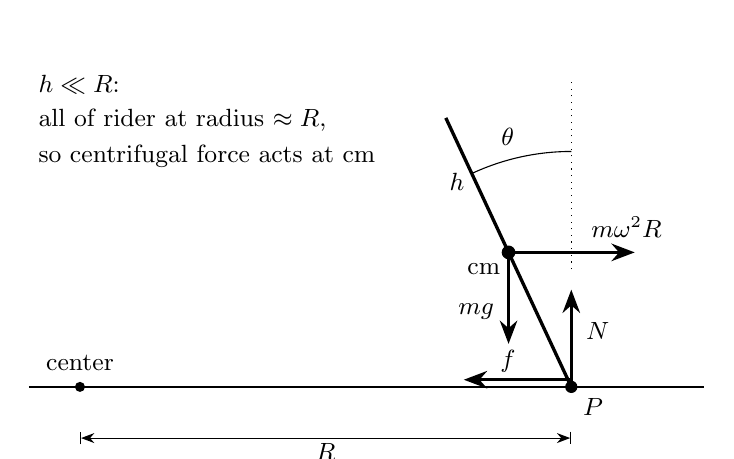
\begin{tikzpicture}[scale=1.3,>=Stealth,font=\small]
  % ground and the track radius, dimensioned below the ground so the two
  % horizontal lines do not sit on top of each other
  \draw[thick] (-5.3,0) -- (1.3,0);
  \fill (-4.8,0) circle (1.4pt);
  \node[above] at (-4.8,0.06) {center};
  \draw[|<->|] (-4.8,-0.5) -- (0,-0.5);
  \node[below] at (-2.4,-0.46) {$R$};
  % vertical reference, started above the normal force so they do not overlap
  \draw[dotted] (0,1.15) -- (0,3.0);
  % the rider
  \draw[very thick] (0,0) -- (-1.226,2.628);
  \node[left] at (-0.95,2.00) {$h$};
  \fill (0,0) circle (1.7pt);
  \node[below right] at (0.02,-0.02) {$P$};
  \draw (0,2.3) arc (90:115:2.3);
  \node at (-0.62,2.44) {$\theta$};
  \fill (-0.613,1.314) circle (1.9pt);
  \node[below left] at (-0.60,1.30) {cm};
  % forces
  \draw[->,very thick] (0,0) -- (0,0.95);
  \node[right] at (0.05,0.55) {$N$};
  \draw[->,very thick] (0,0.07) -- (-1.05,0.07);
  \node[above] at (-0.62,0.05) {$f$};
  \draw[->,very thick] (-0.613,1.314) -- (-0.613,0.42);
  \node[left] at (-0.66,0.74) {$mg$};
  \draw[->,very thick] (-0.613,1.314) -- (0.62,1.314);
  \node[anchor=south west] at (0.10,1.36) {$m\omega^2 R$};
  % the observation that licenses the whole calculation
  \node[anchor=west] at (-5.3,2.95) {$h \ll R$:};
  \node[anchor=west] at (-5.3,2.60) {all of rider at radius $\approx R$,};
  \node[anchor=west] at (-5.3,2.25) {so centrifugal force acts at cm};
\end{tikzpicture}
\end{center}

\ann{$\uparrow$ The diagram is the setup. Every symbol used below ($P$, $\theta$, cm, $R$)
is defined on it, and the first line says which frame we're in.}

\medskip
Let cm be a distance $\ell$ up the rod from $P$. Torque about $P$ (rider is static in this
frame, so $\tau_{\text{net}}=0$; $N$ and $f$ act at $P$ and contribute nothing):

\[ \tau = m\omega^2 R\,(\ell\cos\theta) \;-\; mg\,(\ell\sin\theta) = 0 \]

\ann{$\uparrow$ ``Torque about $P$'' is named, and the reason $N$ and $f$ drop out takes
half a line. This is a rubric line.}

\[ \omega^2 = \frac{g\tan\theta}{R} \]

\sout{$\omega^2 = g\cot\theta / R$ \quad - lever arms swapped} \quad
\ann{$\leftarrow$ First attempt, caught and crossed out. See the check below.}

\medskip
\fbox{$\displaystyle \omega = \sqrt{\frac{g\tan\theta}{R}}$}

\medskip
\emph{Check:} $\theta \to 0$ (upright) $\Rightarrow \omega \to 0$. \checkmark\ \
$\theta \to 90^\circ \Rightarrow \omega \to \infty$. \checkmark\ \ Units: $\sqrt{(\text{m/s}^2)/\text{m}}
= \text{s}^{-1}$. \checkmark

\ann{$\uparrow$ This check is what caught the swapped lever arms. It took three lines and
maybe thirty seconds, and it's the difference between 8/8 and 3/8 on this part.}

\end{sheet}

\begin{sheet}{Student AAPT ID \#\qquad Proctor AAPT ID \#\\ A1 -- 2/2}

\textbf{(b)} \quad Now $h \not\ll R$, so different parts of the rod are at different radii
and the centrifugal force is \emph{not} uniform.

\medskip
\sout{Idea: cm sits at radius $R - \tfrac{h}{2}\sin\theta$, so replace $R \to R -
\tfrac{h}{2}\sin\theta$ in (a).}

\ann{$\leftarrow$ The trap, tried and abandoned. There's a one-line reason written next to
it instead of a silent erasure:}

\smallskip
\emph{No - torque involves the product $r\,z$, and $\langle rz\rangle \neq \langle r
\rangle\langle z\rangle$. Must integrate.}

\medskip
\textbf{Setup.} Mass element a distance $s$ along the rod from $P$:
\[ r = R - s\sin\theta, \qquad z = s\cos\theta, \qquad dm = \frac{m}{h}\,ds,
\qquad 0 \le s \le h \]

\ann{$\uparrow$ Each of these three is a rubric line on its own. Even if the integral had
gone nowhere, these already get points.}

\medskip
\textbf{Centrifugal torque about $P$.} Force $\omega^2 r\,dm$ outward, lever arm $z$:
\[ \tau_c = \int_0^h \omega^2 (R - s\sin\theta)(s\cos\theta)\,\frac{m}{h}\,ds \]

\[ = \frac{m\omega^2\cos\theta}{h}\left[ \frac{Rh^2}{2} - \frac{h^3\sin\theta}{3} \right]
 = m\omega^2 h\cos\theta \left( \frac{R}{2} - \frac{h\sin\theta}{3} \right) \]

\textbf{Gravity torque about $P$}, at the cm, $h/2$ up the rod:
\[ \tau_g = -\,mg\,\frac{h}{2}\sin\theta \]

\textbf{Balance.} $\tau_c + \tau_g = 0$:
\[ \omega^2 h\cos\theta\left( \frac{R}{2} - \frac{h\sin\theta}{3}\right)
   = g\,\frac{h}{2}\sin\theta
   \quad\Longrightarrow\quad
   \omega^2 = \frac{g\tan\theta}{R - \tfrac{2h}{3}\sin\theta} \]

\medskip
\fbox{$\displaystyle \omega = \sqrt{\frac{g}{R}\tan\theta \left(1 - \frac{2h}{3R}\sin\theta
\right)^{-1}}$}

\medskip
\emph{Checks:} $h \to 0$ reduces to (a) \checkmark\ \ Denominator $< R$, so $\omega$ is
\emph{larger} than in (a) \checkmark\ - correct, since the rod's mass sits at smaller
radius than $R$ and so needs a faster spin to hold the lean.

\ann{$\uparrow$ Two lines of checks. The first shows the correction is consistent with (a),
and the second shows the sign of the correction was understood, not just stumbled into.}

\end{sheet}

% Break here so the rubric table lands whole on one page; a two-row orphan with
% a "(continued)" header is exactly the thing this section is arguing against.
\pagebreak

\subsection*{How that gets graded}

USAPhO rubrics aren't published, so the breakdown below is a reconstruction, but it has the
right shape: a 25-point problem is cut into five or six milestones, and each one is awarded
on its own.

\begin{center}
\begin{longtable}{p{0.60\textwidth}cc}
\hline
\textbf{Rubric line} & \textbf{Pts} & \textbf{Earned} \\
\hline
\endfirsthead
\multicolumn{3}{l}{\emph{(continued)}} \\
\hline
\textbf{Rubric line} & \textbf{Pts} & \textbf{Earned} \\
\hline
\endhead
\multicolumn{3}{l}{\textbf{(a) Point-mass limit}} \\
Correct force picture: states the frame and identifies the centrifugal force acting at
the cm & 2 & 2 \\
Correct torque (or force) balance about the contact point & 3 & 3 \\
Correct $\omega = \sqrt{g\tan\theta/R}$ & 3 & 3 \\
\hline
\multicolumn{3}{l}{\textbf{(b) Extended rod}} \\
Recognizes the centripetal acceleration varies along the rod, so the cm substitution
fails & 3 & 3 \\
Correct parametrization $r = R - s\sin\theta$, $z = s\cos\theta$, $dm = (m/h)ds$ & 4 & 4 \\
Correct integral expression for the centrifugal torque & 4 & 4 \\
Correct evaluation $m\omega^2 h\cos\theta\!\left(\tfrac{R}{2} - \tfrac{h\sin\theta}{3}\right)$
& 3 & 3 \\
Correct gravitational torque and balance & 3 & 3 \\
Correct final $\omega$, boxed & 3 & 3 \\
\hline
\textbf{Total} & \textbf{25} & \textbf{25} \\
\hline
\end{longtable}
\end{center}

That submission gets full marks, and notice how little of the page is polished. There's a
crossed-out formula, an abandoned idea, and no prose beyond a few six-word fragments. It
gets a 25 because every rubric line can be found in under ten seconds.

\subsection*{The same physics, written four other ways}

Here's what separates scores on this exam. All four of these students did roughly the same
amount of physics.

\begin{center}
\begin{longtable}{p{0.62\textwidth}c}
\hline
\textbf{What the page contains} & \textbf{Score} \\
\hline
\endhead
\textbf{Ran out of time in (b).} Part (a) complete. In (b): ``the centripetal acceleration
varies along the rod, so I have to integrate the torque instead of using the cm,'' plus
$r = R - s\sin\theta$, $z = s\cos\theta$, $dm = (m/h)ds$, and the integral written down but
never evaluated. & \textbf{18/25} \\[4pt]
\textbf{Fell into the trap.} Part (a) complete. In (b), substituted $R \to R -
\tfrac{h}{2}\sin\theta$ with no comment and boxed it. & \textbf{9/25} \\[4pt]
\textbf{Blew part (a), recovered.} Part (a) has the lever arms swapped and is never checked,
so $\cot\theta$ is boxed. Part (b) is done correctly from scratch, with the setup, integral,
evaluation, balance, and answer all there. & \textbf{22/25} \\[4pt]
\textbf{Did all the physics, wrote none of it.} Everything correct, but done on scratch
paper, with only the two boxed answers copied onto the answer sheets. & \textbf{6/25} \\
\hline
\end{longtable}
\end{center}

\begin{keybox}
The third student got \emph{part (a) wrong} and still scored 22, because subparts are graded
independently and (b) was written out. The fourth student solved the whole problem correctly
and scored 6, because the work was on the wrong paper.

The difference between 6 and 22 here has nothing to do with physics. It comes from where you
wrote and how you labeled it.
\end{keybox}

\subsection*{Things that go wrong, and what to do about them}

\Q{You suspect part (a) is wrong but can't see why.}
Run the limiting cases. That's what caught the swapped lever arms above. Set each parameter
to zero or infinity in turn and ask whether the answer still makes sense. If a check fails,
you've found a real error in thirty seconds. If they all pass, stop worrying and move on. A
wrong (a) doesn't sink (b) anyway.

\Q{You can't see how to set up the integral in (b).}
Write down what you \emph{do} know (``the acceleration varies along the rod, so
$\tau_c = \int \omega^2 r z \, dm$'') and then define $r$, $z$, and $dm$ one at a time
against your diagram. That setup alone gets 7 of the 17 points in (b), before you've
integrated anything. A lot of the time, being stuck means trying to write the whole setup
in one line.

\Q{You get an ugly answer and think you must have made a mistake.}
Ugly answers are normal. $\omega^2 = g\tan\theta/(R - \tfrac{2h}{3}\sin\theta)$ is ugly,
and it's correct. Check the limits, box it, and move on. Don't spend ten minutes hunting for
a mistake that isn't there just because you expected something prettier.

\Q{You have two versions of an answer and no time to decide.}
Pick the one that passes your limiting checks, box it, and put a single line through the
other one. Don't leave both standing.

\Q{You're 30 minutes in with (b) half done.}
Stop. Box whatever you have, write one line saying what's left (``still need to evaluate
the integral and balance against gravity''), and go read the next problem. Its first
subpart is probably worth more points than your next ten minutes on this one.

\section{Part VI: Two Real Papers}

Everything so far has been a made-up example. These two are real. Both pages below are
actual 2018 USAPhO submissions to Problem B2, reproduced as the graders received them, with
the scores they actually got. The scans only carry the AAPT numbers printed on the answer
sheet; there are no names on them.

\begin{official}
\textbf{Question B2 (2018 USAPhO).} In this problem, use a particle-like model of photons:
they propagate in straight lines and obey the law of reflection, but are subject to the
quantum uncertainty principle. You may use small-angle approximations throughout.

A photon with wavelength $\lambda$ has traveled from a distant star to a telescope mirror,
which has a circular cross-section with radius $R$ and a focal length $f \gg R$. The path of
the photon is nearly aligned to the axis of the mirror, but has some slight uncertainty
$\Delta\theta$. All small cross-sectional areas of the mirror are equally likely to include
the point of reflection.

\begin{subpart}
\item Find the standard deviation $\sigma_r$ of the distribution for $r$, the distance from
the center of the mirror to the point of reflection.
\item Use the uncertainty principle, $\sigma_r \sigma_{p_r} \ge \hbar/2$, to place a bound on
how accurately we can know the angle of the photon from the axis of the telescope. Give your
answer in terms of $R$ and $\lambda$. \emph{If you were unable to solve part a, you may also
give your answer in terms of $\sigma_r$.}
\item Suppose we want to tell with high probability whether a detected photon came from the
left half or right half of Alpha Centauri A. Approximately how large would the telescope
have to be? The star is about $4\times10^{16}$ m away with radius about $7\times10^{8}$ m;
assume $\lambda = 500$ nm.
\end{subpart}
\end{official}

Look at the italicized sentence in part (b). The exam is telling you, in writing, that you
can use the move from Part II. Watch which of these two students takes the offer.

\subsection*{Paper 1: 22 out of 25}

\begin{center}
\fbox{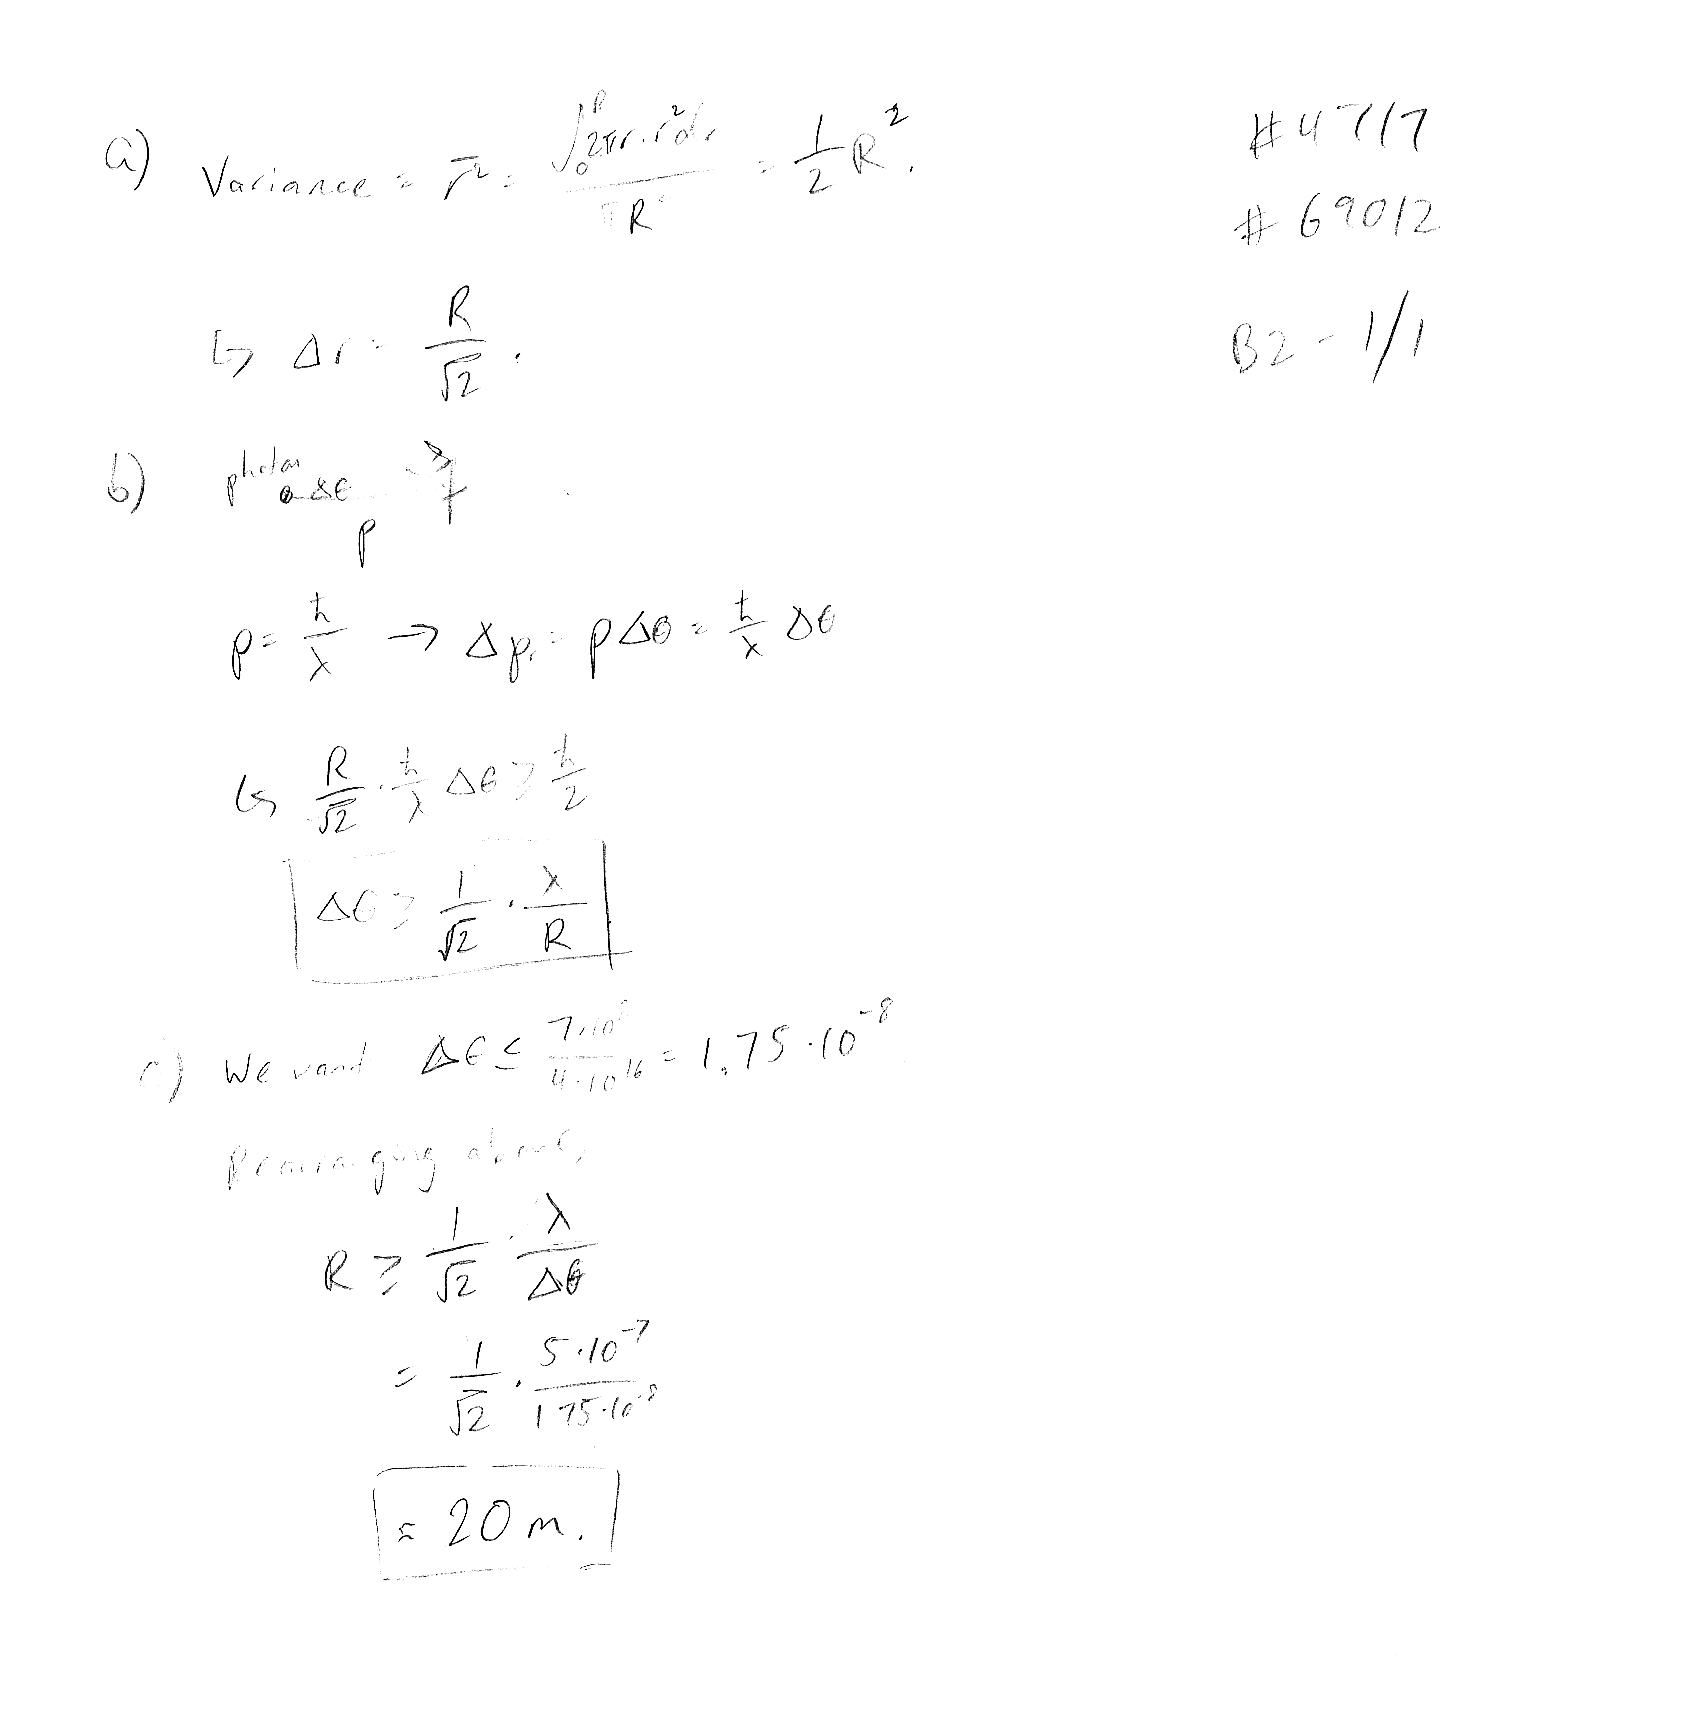
\includegraphics[width=0.86\textwidth]{paper-4717-b2.png}}
\end{center}

\textbf{What they did.} All of B2 on one side of one sheet, headed \textsf{B2 -- 1/1}. In
(a) they wrote the area-weighted average straight down,
$\int_0^R 2\pi r\cdot r^2\,dr\,/\,\pi R^2 = \tfrac{1}{2}R^2$, and took the square root. In
(b) they sketched the photon and the angle, wrote $p = \hbar/\lambda$ and
$\Delta p_r = p\,\Delta\theta$, put those into the uncertainty relation, and boxed
$\Delta\theta \ge \tfrac{1}{\sqrt2}\,\lambda/R$. In (c) they got the angle the telescope has
to resolve, $7\times10^{8} / 4\times10^{16} = 1.75\times10^{-8}$, rearranged their own (b)
for $R$, and boxed about 20 m.

\textbf{Why they got the credit they did.} Each subpart is a short chain a grader can follow
start to finish in a few seconds, and both final answers are boxed. Part (a) is actually
wrong: they computed the root-mean-square radius, not the standard deviation. With
$\langle r\rangle = 2R/3$, the variance is $\langle r^2\rangle - \langle r\rangle^2 =
R^2/18$, so $\sigma_r = R/(3\sqrt2)$, smaller than what they wrote by a factor of three.
They lost the points for (a) and kept nearly everything else, because (b) and (c) were
carried through correctly \emph{from their own} (a). This is normal. Graders mark
consequentially, so a later part done right using a wrong earlier number still gets the
later points.

\textbf{What would have earned more.} Only that one thing. Writing down the definition they
were using, $\sigma^2 = \langle r^2\rangle - \langle r\rangle^2$, before computing anything
would probably have caught it, since the missing $\langle r\rangle^2$ term is visible as
soon as the formula is on the page. Naming the principle first helps the grader, and it's
also how you catch your own mistakes.

\subsection*{Paper 2: 5 out of 25}

\begin{center}
\fbox{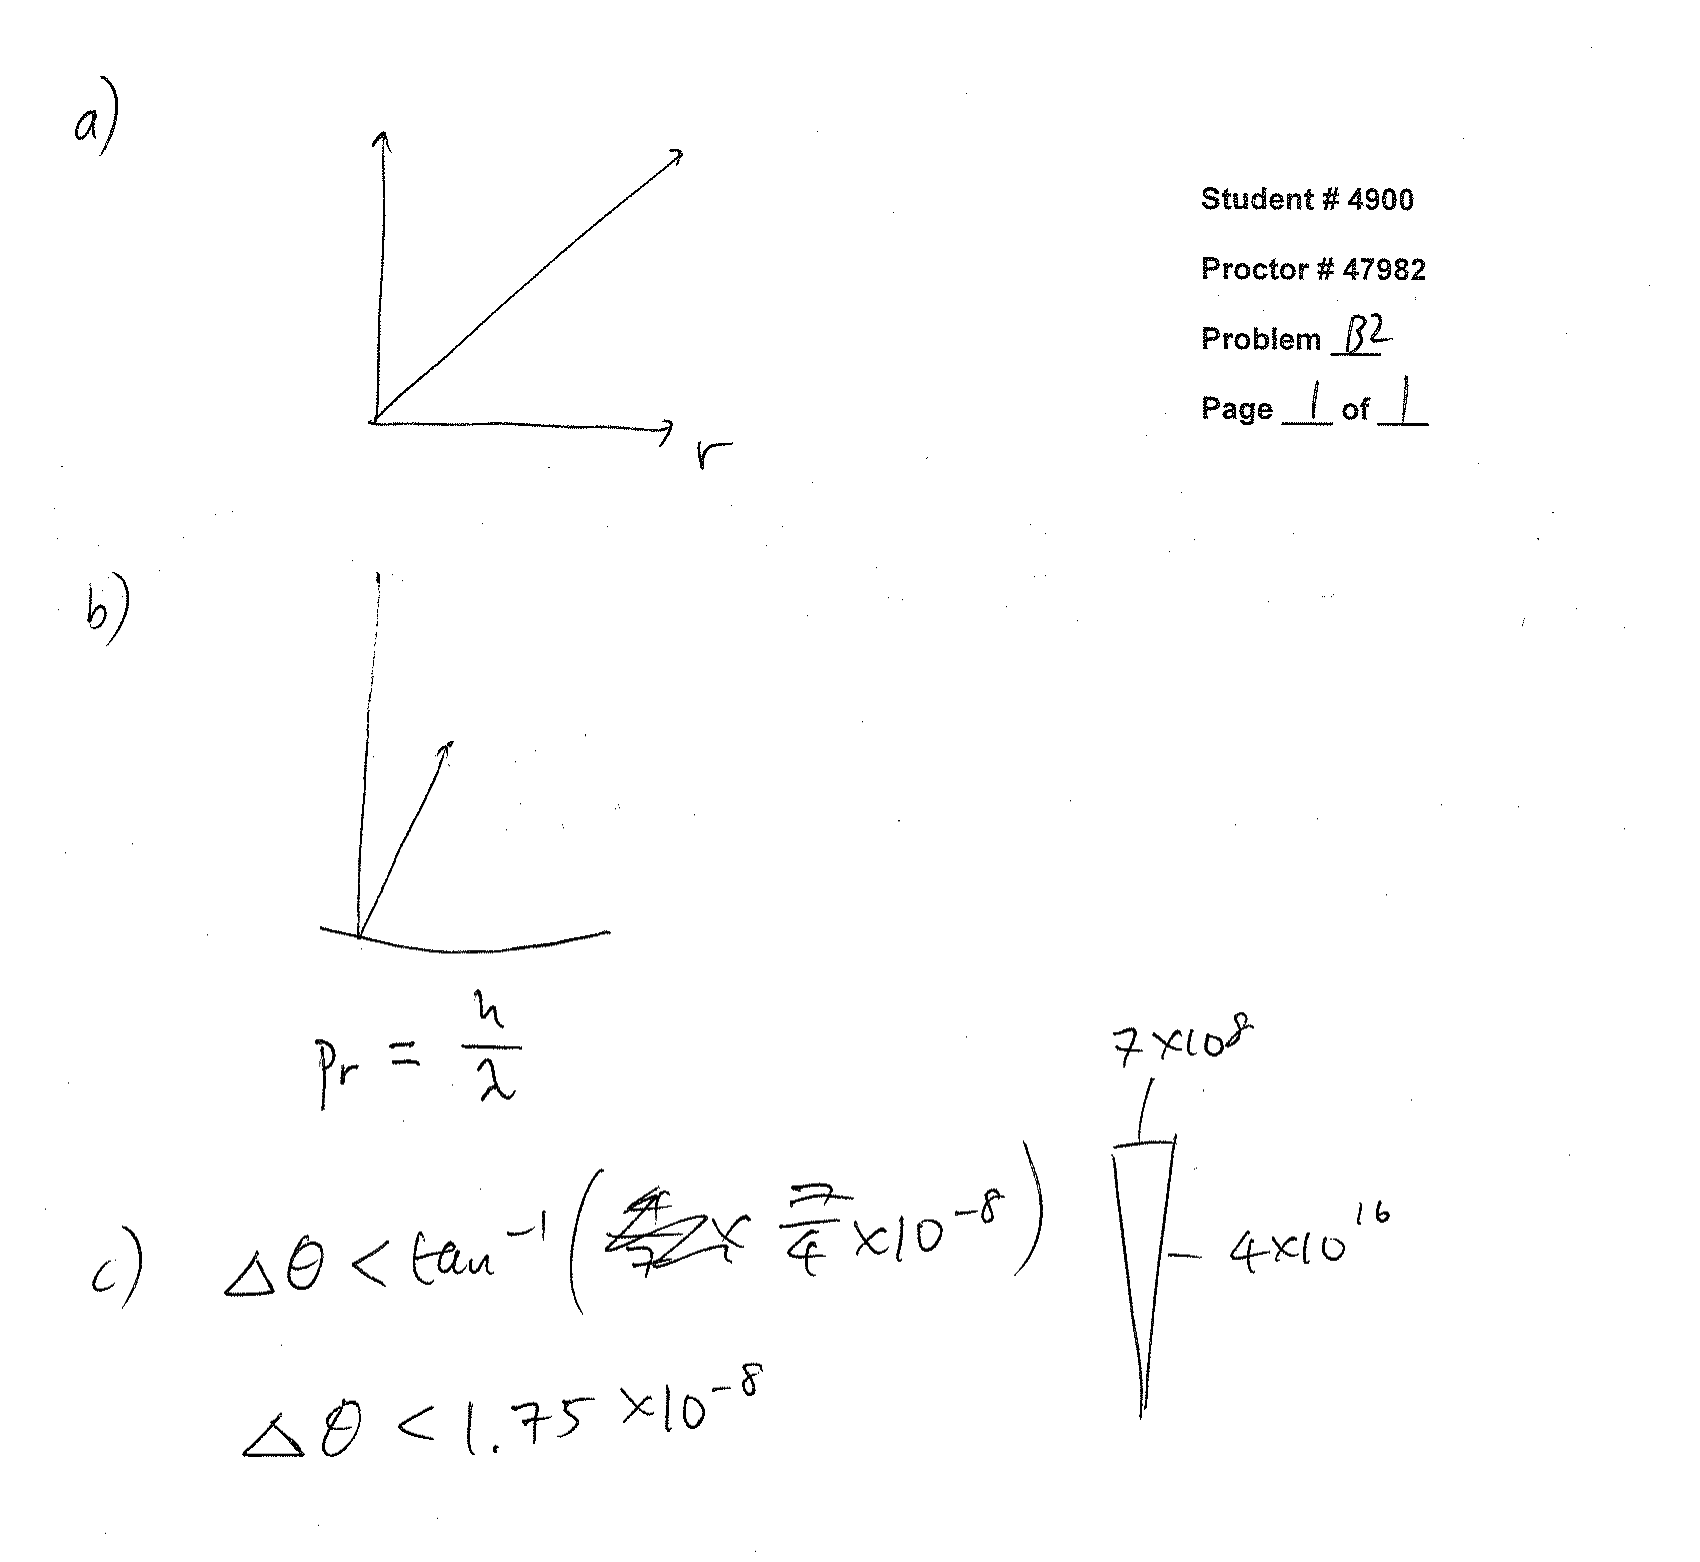
\includegraphics[width=0.86\textwidth]{paper-4900-b2.png}}
\end{center}

Before you read this as a weak paper: the same student scored 25/25 on A1 and 23/25 on A3
that day, and A3 was the problem where 45\% of the field scored zero. This student knew
plenty of physics.

\textbf{What they did.} In (a), a pair of axes labeled $r$ with an arrow across them, and no
distribution, integral, or answer. In (b), a sketch of a photon hitting the mirror and a
single equation, $p_r = h/\lambda$. In (c), a sketch of the star and the angle it subtends
at Earth, and $\Delta\theta < \tan^{-1}(\tfrac{7}{4}\times10^{-8}) = 1.75\times10^{-8}$.

\textbf{Why they got the credit they did.} Two of the three physical ingredients on that
page are right, and they're the same two Paper 1 used: the photon momentum $h/\lambda$, and
the angular size of Alpha Centauri A. That's what the 5 points are for. But nothing on the
page connects them. Part (b) never uses the uncertainty principle it asked about, so no
bound on $\Delta\theta$ ever shows up. Part (c) finds the angle the telescope has to resolve
and stops there, but the question asked how big the telescope has to be, and no size is
ever computed. Nothing is boxed.

\textbf{What would have earned more.} Three lines, and none of them needed an idea this
student didn't already have on the page:

\begin{itemize}\setlength{\itemsep}{2pt}
\item \textbf{Take the offer in part (b).} The problem says outright that you can answer in
terms of $\sigma_r$. Writing $\sigma_r \cdot \tfrac{h}{\lambda}\Delta\theta \ge \hbar/2$
and solving for $\Delta\theta$ needs nothing from part (a), and $p = h/\lambda$ was already
written down two inches above.
\item \textbf{Finish (c) with what you have.} Even with no bound from (b), $R \sim
\lambda/\Delta\theta = 5\times10^{-7} / 1.75\times10^{-8} \approx 30$ m is one division,
and it answers the question that was asked. An order-of-magnitude answer gets credit. A
correct intermediate quantity that stops short of the question doesn't get much.
\item \textbf{Put a sentence next to each sketch.} Three of the marks on this page are
drawings with nothing written next to them. The (c) sketch has exactly the right idea in it
(the star's radius over its distance is the angle you need to resolve), but a grader can
only give credit for reasoning they can identify, and five words would have turned that
doodle into reasoning.
\end{itemize}

\begin{keybox}
Both students had the same two facts on the page. One turned them into two boxed numbers
and scored 22. The other left them as unconnected marks and scored 5. The difference wasn't
how much physics they knew.

This isn't a story about one unlucky paper, either. B2's mean score was 5.0 out of 25, and
52\% of the field scored zero on it. Paper 2 is a completely typical B2 submission, and the
exam had told every one of those students, right in the text of part (b), how to get past
the step that stopped them.
\end{keybox}

\section{Checklist}

\begin{keybox}
\textbf{Before the exam}
\begin{enumerate}\setlength{\itemsep}{2pt}
\item[$\square$] Confirmed the date, start time, and site with your proctor
\item[$\square$] Non-graphing scientific calculator, memory cleared
\item[$\square$] Memorized the formulas the reference sheet doesn't give you (it's constants
and four approximations, nothing else)
\item[$\square$] Practiced on at least two past USAPhOs under timed conditions, writing on
paper, in 90-minute blocks
\end{enumerate}

\textbf{During the exam}
\begin{enumerate}\setlength{\itemsep}{2pt}
\item[$\square$] Read all three problems before starting any of them
\item[$\square$] Diagram first, symbols defined on it
\item[$\square$] Name the principle before the algebra
\item[$\square$] Symbols throughout; numbers only at the end
\item[$\square$] Box every subpart's final answer
\item[$\square$] Header on every page: problem number and $n/N$
\item[$\square$] Solve on the answer sheets, not on scratch paper
\item[$\square$] Stuck? Write down an assumed result and do the next part anyway
\item[$\square$] 30 minutes per problem, then stop
\item[$\square$] Last four minutes: box, label, cross out, sort
\end{enumerate}
\end{keybox}

\vspace{0.5em}
\begin{center}
\emph{If you have questions this handout doesn't answer, ask me. And check
\href{https://www.aapt.org/physicsteam/}{aapt.org/physicsteam}, which always has the final
say.}
\end{center}

\end{document}
